
\begin{frame}{Citeren-stijl}
	% Bij bibliografie\"en is er een wildernis aan verschillende stijlen:
	Verschillende stijlen zijn mogelijk, onder meer:
	
	\begin{itemize}
		\item \mintinline{tex}|numeric|: This is well-known [2], but also controversial [5, 6].\par
		%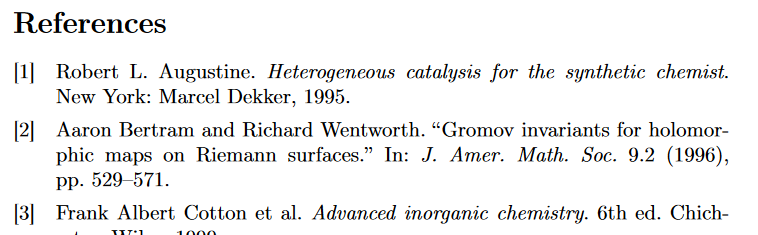
\includegraphics[width=0.8\textwidth]{bib/assets/biblatexStyles/numericReferences.png}
		
		\item \mintinline{tex}|alphabetic|: This is well-known [GMS94], but also controversial [Gon01, Ham97].
		\item \mintinline{tex}|authoryear|: This is well-known John 2003, ...
		\item \mintinline{tex}|apa|: This is well-known (Lambert, 1993), bb ...
	\end{itemize}
	In APA: \mintinline{tex}|\cite| en \mintinline{tex}|\parencite| verschillen
\end{frame}

\begin{saveblock}{codebox}
	%\highlightC{style=numeric}%
	\begin{minted}{tex}
		\usepackage[style=numeric]{biblatex}
	\end{minted}
\end{saveblock}


\begin{saveblock}{codeboxD}%
	\begin{minted}{tex}
		\DeclareLanguageMapping{english}{english-apa}
	\end{minted}
\end{saveblock}

\begin{frame}{Citeren-stijl}
	%En er zijn nog veel meer stijlen!
	Voor exacte wetenschappen: gebruik numeric. Zo
	verander je de stijl:
	\useblock{codebox}
	
	\medskip
	Voor APA-stijl heb je daarnaast nodig:
	\useblock{codeboxD}
	In de preamble van het template staan de verschillende stijlen met uitgebreide uitleg
\end{frame}
